\section{Discussion}
\label{sec:discussion}

We now reflect on our work by elaborating on its shortcomings
(\Cref{sec:biases}) and proposing future research directions
(\Cref{sec:future-work}).

\subsection{Biases}
\label{sec:biases}

A truly uniform sample of Tor users is difficult to obtain.  One strategy would
have been to work with The Tor Project to add a link to our experiment on Tor
Browser's landing page.  While this approach would have reached a large number
of Tor users, we considered it prohibitively invasive.  Besides, people who
rarely restart their Tor Browser or pay no attention to the landing page would
have still missed our experiment.  We therefore decided to ask The Tor Project
to disseminate our survey on its blog and Twitter account.  We believe that this
recruitment strategy was subject to the following biases.

\textbf{Non-response bias}:
People who noticed our call for volunteers but decided against participating may
have valued their privacy too much, falsely believed that their perspective is
irrelevant, lacked time, or had other reasons not to participate.  Nevertheless,
non-respondents may exhibit traits that are fundamentally different from those
who did participate, which is why their absence in our sample may bias our
results.

\textbf{Survivor bias}:
We predominantly heard from people who can tolerate Tor Browser's usability
issues, which is why they are still around to tell their tale.  We likely did
not hear from many---if any---people who decided that Tor Browser was not for
them and were thus unable to tell us what drove them away.  The danger of
survivor bias lies in optimizing the user experience for the subset of people
whose tolerance for inconvenience is higher than the rest.

\textbf{Self-selection bias}:
Due to the nature of our online survey, participants could voluntarily select
themselves into our set of respondents.  These respondents may be unusually
engaged and technical, which is why they have formed opinions that they consider
worth sharing.  Indeed, the demographic for our online survey in
\Cref{sec:online-survey} was rather young and educated---but perhaps Tor
Browser's population \emph{is} young and educated.

\subsection{Future Work}
\label{sec:future-work}

The Tor Project is currently working on a security indicator for onion
services~\cite{trac23247}.  \Cref{fig:onion-service} illustrates that Tor
Browser currently, in version 7.0.10, displays an onion service connection like
a plain \textsc{http} connection, thus greatly ``underselling'' the security and
privacy that an onion service connection provides.  The work of Porter Felt
\ea~\cite{Felt2016a} revealed the subtleties that one must consider when
designing security indicators, which highlights the importance of an independent
study of an onion connection security indicator.  Do users correctly understand
the meaning of an onion service indicator?  Do they also understand how it
differs from an \textsc{https} indicator?  Tor Browser's circuit display
\textsc{ui} (see \Cref{fig:tor-button}) is currently experiencing a
redesign~\cite{trac24309}.  Similar to the onion service indicator, an empirical
evaluation of the circuit display could reveal user misunderstandings.  For
example, some users are not familiar with the concept of guard relays and
incorrectly expect each relay in their circuit to change.

\begin{figure}[t]
    \centering
    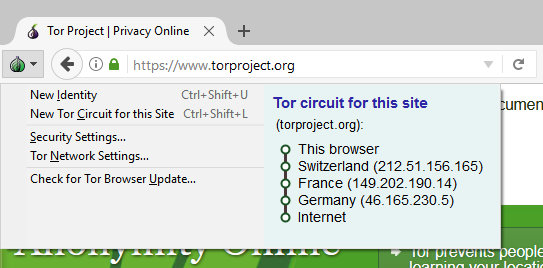
\includegraphics[width=\linewidth]{figures/tor-button-screenshot.jpg}
    \caption{A click on the onion icon reveals the Tor relays that constitute
    the circuit that was used to fetch the current page.  As of February 2018,
    the user interface is subject to a redesign~\cite{trac24309}.}
    \label{fig:tor-button}
\end{figure}

Our survey results suggest that there is a need for a system that automates
onion service discovery, \eg, by providing an opt-in mechanism that
automatically publishes onion domains in a public log, allowing users to learn
about new onion domains as they are added to the log.  An orthogonal usability
improvement would be transparent ``upgrading'' from a web site to its
corresponding onion service.  The Tor Project is currently investigating the
problem space on its bug tracker~\cite{trac21952}.  Finally, our survey
responses suggest that there is a need for a privacy-preserving bookmarking tool
that allows users to bookmark sites without leaving a browsing trail on their
hard drives.
